\documentclass[a4paper]{article}

\usepackage[T1]{fontenc}
\usepackage[utf8x]{inputenc}

\usepackage[a4paper]{geometry}
\geometry{verbose,tmargin=3cm,bmargin=3cm,lmargin=2cm,rmargin=2cm,headheight=2cm,headsep=1cm,footskip=2cm}


\usepackage{fancyhdr}
\usepackage{enumerate}
\usepackage{adjustbox}
\pagestyle{fancy}
\setlength{\parskip}{\medskipamount}
\setlength{\parindent}{0pt}
\usepackage{graphicx}

\makeatletter

\usepackage{subcaption}
\usepackage{varwidth}
\usepackage{float} 
\usepackage{color}
\usepackage{lastpage}
\usepackage{indentfirst}

\usepackage{pgf}
\usepackage{tikz}
\usetikzlibrary{arrows,automata, shapes, positioning, calc}

\lhead[lh-even]{Edgar Vedvik (edgarmv)}
\chead[ch-even]{TTM4135 Information Security}
\rhead[rh-even]{\today}

\lfoot[lf-even]{}
\cfoot[cf-even]{Page \thepage{} of \pageref{LastPage}}
\rfoot[rf-even]{}

\date{}

\makeatother

\usepackage[english]{babel}

\begin{document}
\thispagestyle{fancy}

\section{Analyse the ciphertext histograms}

    Below I have plotted the histograms for each file and figured out their corresponding cipher.

    \subsection{File 0.txt - Transposition}

        \begin{figure}[h]
            \centering
            \begin{subfigure}{.5\textwidth}
                \centering
                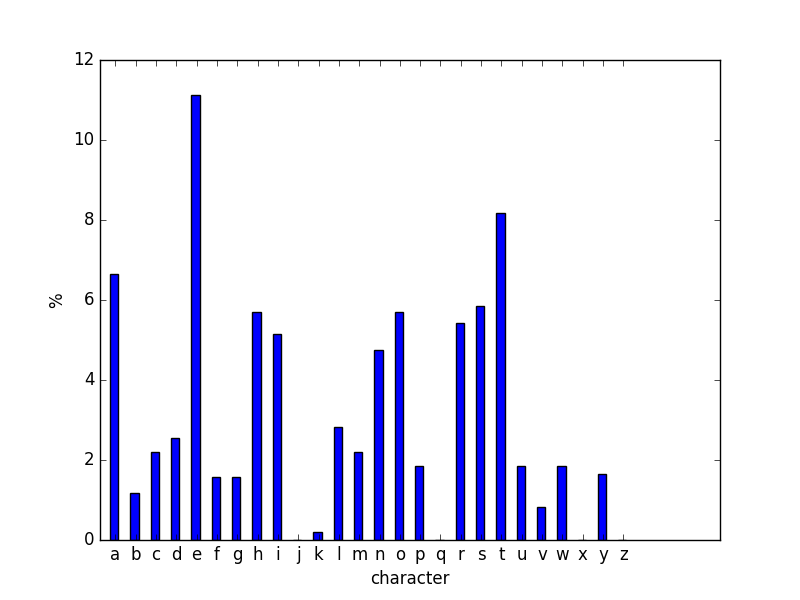
\includegraphics[width=1\textwidth]{histogram_0.png}
                \caption{Ciphertext}
            \end{subfigure}%
            \begin{subfigure}{.5\textwidth}
                \centering
                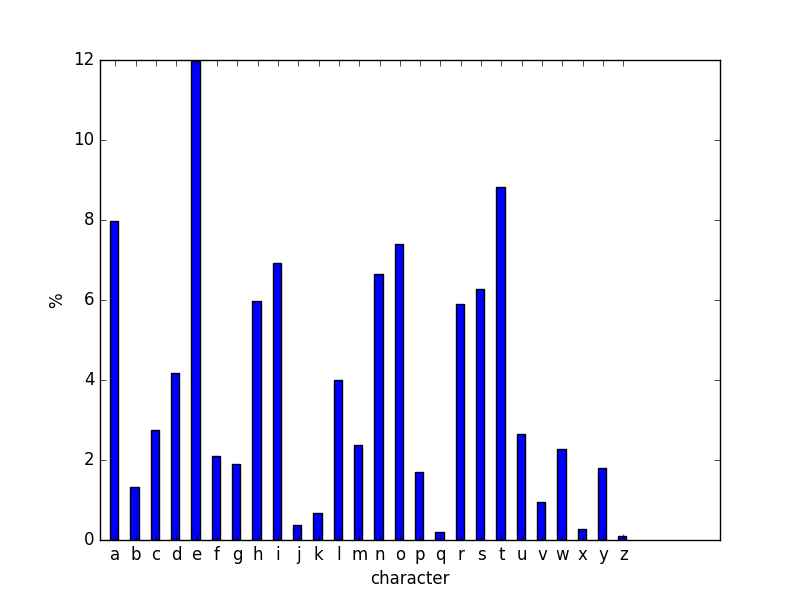
\includegraphics[width=1\textwidth]{histogram_english.png}
                \caption{English}
            \end{subfigure}
            \caption{Histograms for the transposition cipher}
        \end{figure}

        The character frequency in the ciphertext is the same as that of a standard english text.
        This points to a transposition cipher, which preserves the character frequency in the
        encrypted text

    \subsection{File 1.txt - Random simple substitution}

        \begin{figure}[h]
            \centering
            \begin{subfigure}{.5\textwidth}
                \centering
                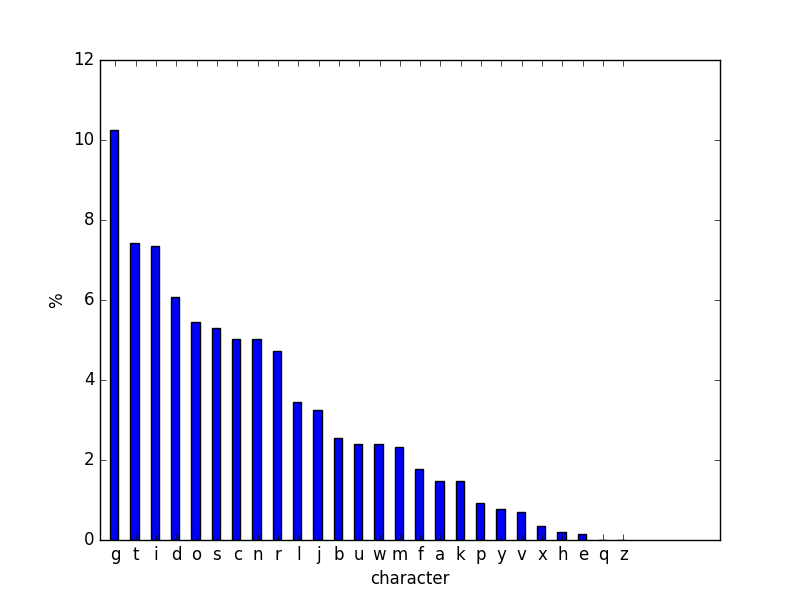
\includegraphics[width=.9\textwidth]{histogram_sorted_1.png}
                \caption{Ciphertext}
            \end{subfigure}%
            \begin{subfigure}{.5\textwidth}
                \centering
                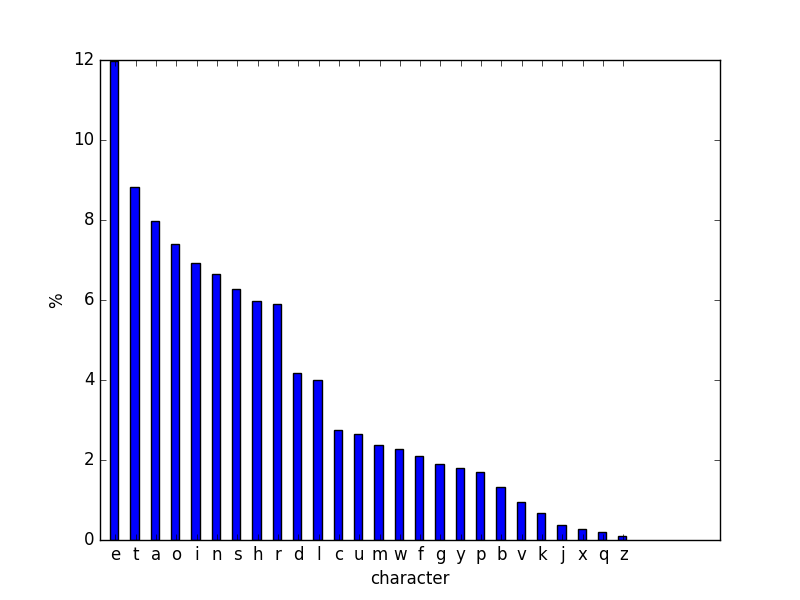
\includegraphics[width=.9\textwidth]{histogram_sorted_english.png}
                \caption{English}
            \end{subfigure}
            \caption{Histograms for the substitution cipher}
        \end{figure}

        If we sort the histograms by frequency and compare it with a sorted version of the
        english language, we can see that same frequencies appear, just at other characters.
        This points to a simple substitution cipher.


    \subsection{File 3.txt - Vigenère}
        \begin{figure}[h!]
            \centering
            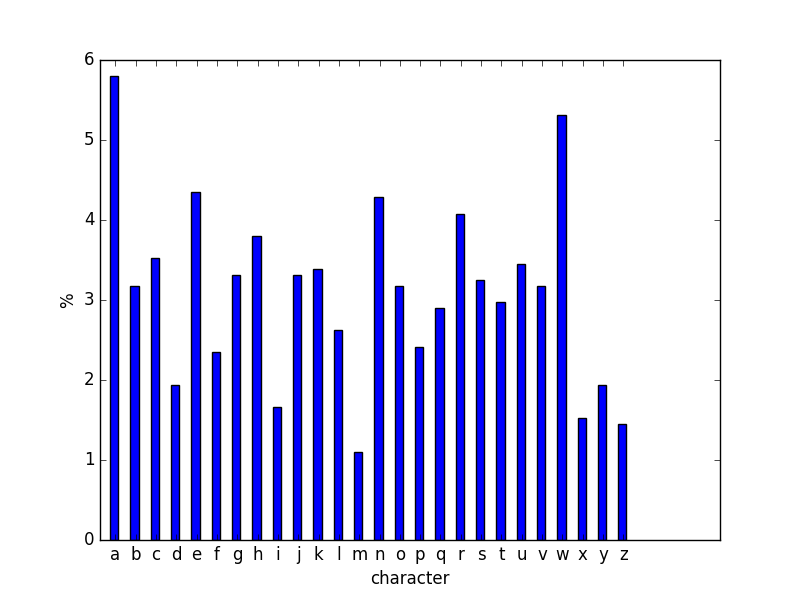
\includegraphics[width=0.75\textwidth]{histogram_3.png}
            \caption{Histogram of the Vigenère cipher}
            \label{fig:histogram3}
        \end{figure}


        This histogram is much more smoothed out than the histograms for the previous ciphers. This
        points to polyalphabetic substituion, which could be either the Vigenère or the Hill cipher.
        However, plotting the autocorrelation of the ciphertext yields Figure 
        \ref{fig:autocorrelation}, which shows us that this is the Vigenère cipher with period 7.

        \begin{figure}[h!]
            \centering
            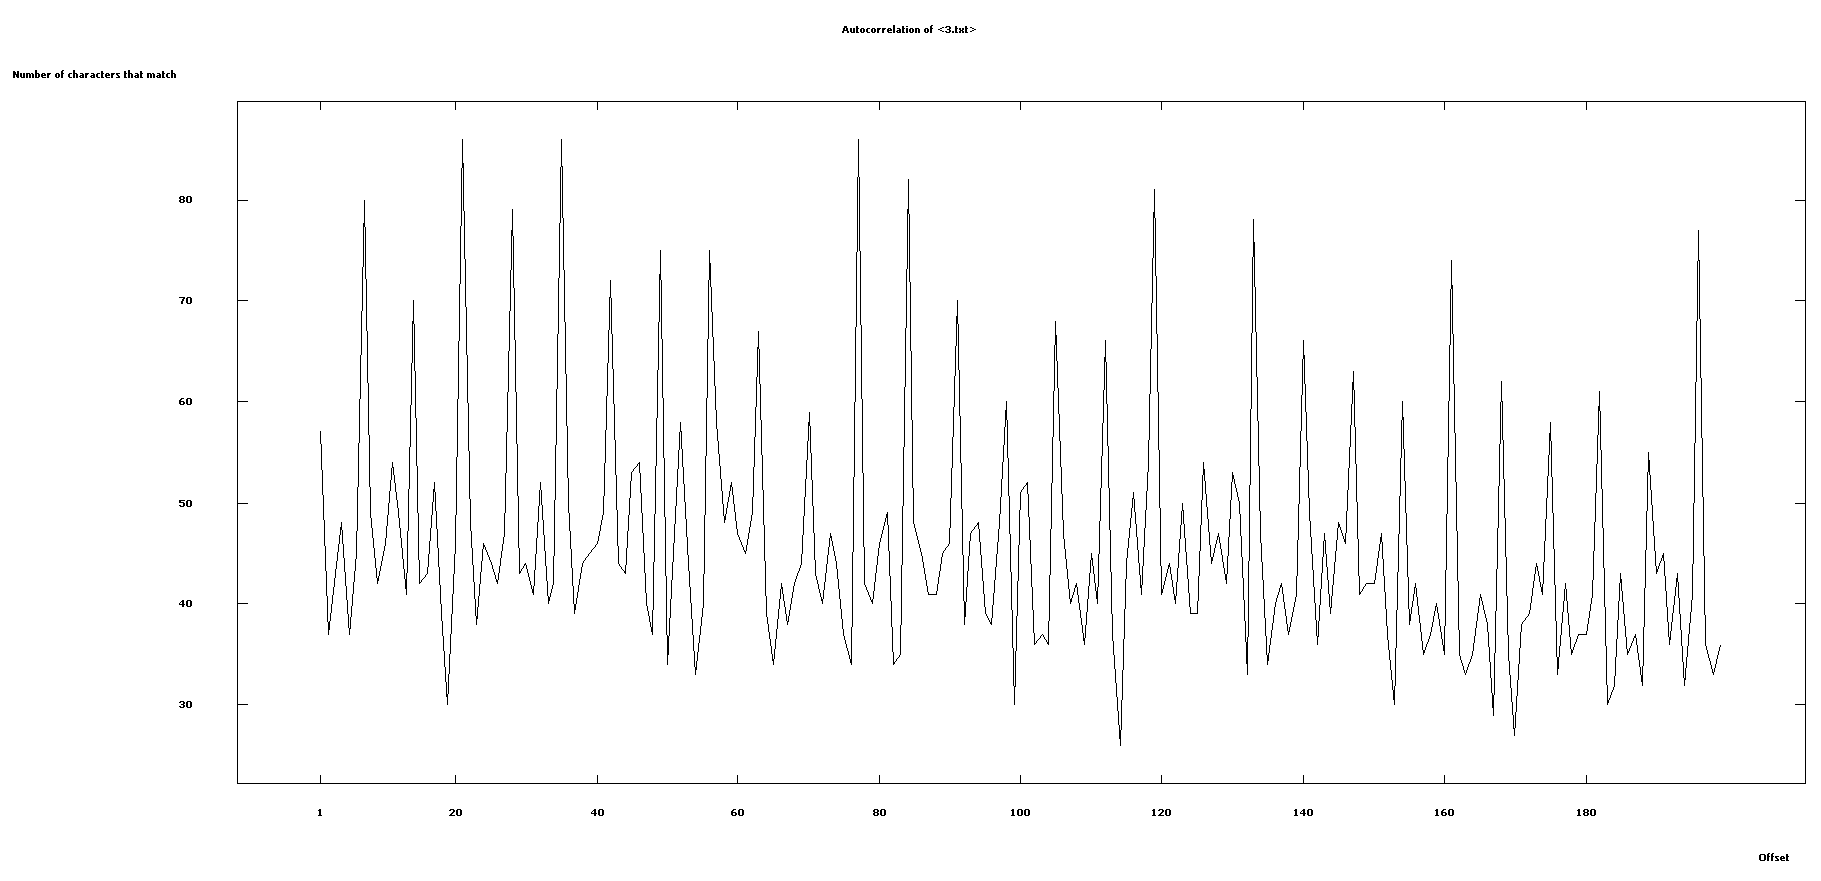
\includegraphics[width=0.95\textwidth]{autocorrelation.png}
            \caption{Autocorrelation of the Vigenère cipher}
            \label{fig:autocorrelation}
        \end{figure}

    \subsection{File 2.txt - 2x2 Hill cipher}

        \begin{figure}[h]
            \centering
            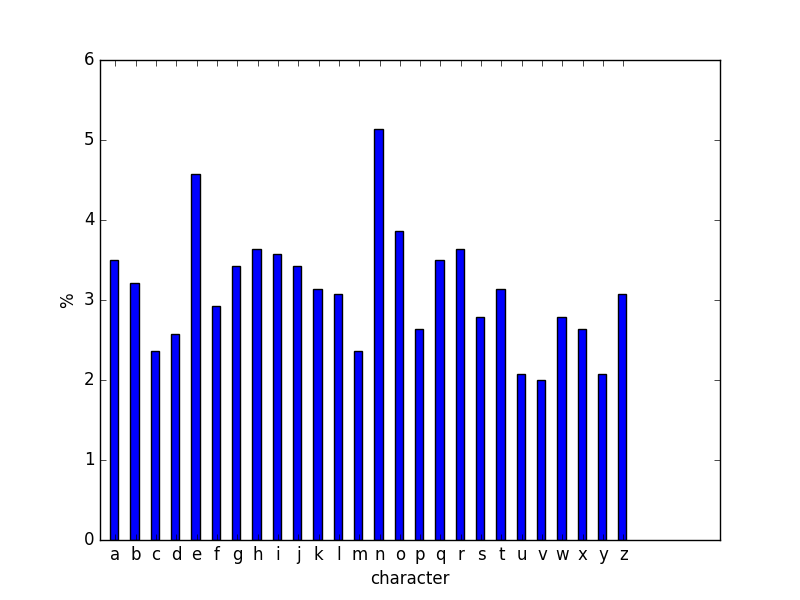
\includegraphics[width=0.75\textwidth]{histogram_2.png}
            \caption{Histogram for the 2x2 Hill cipher}
        \end{figure}

        This cipher also has an even distribution, but since we have only 1 cipher left, this must be
        the 2x2 Hill cipher.

\section{Obtaining the substitution, Vigenère, and transposition plain-texts}

    \subsection{Random simple substitution}
        
        \begin{description}
            \item[key:] IABJGFKCDEHLMNOPQRSTUVWXYZ
            \item[plain-text:] control of the sea was actually at stake. Nor did Admiral Jellicoe
            indulge in any false expectations concerning the future. Bad as the situation 
            then was, he had every expectation that it would grow
        \end{description}

    \subsection{Vigenère}

        \begin{description}
            \item[key:] WNCOJAS
            \item[plain-text:] SUbMergEd fOR a PERiOd, whIle The cRew Of iTS VicTiM Was getTINg
                Off IN boaTs; IT Then caMe tO The SUrface, aNd The MEN pRepaRed To bOaRd The
                dISabled ShiP and SeaRch hER fOR vaLUableS aNd delIcacies
        \end{description}

    \subsection{Transposition}
        \begin{description}
            \item[key:] 7165243.
            \item[plain-text:] for prisoners or the ship s papers  the boats  crews  therefore
                had instructions to take up a station on a bearing from which the ship s guns
                could most successfully rake the submarine  That this manoeuvre involved great
        \end{description}

\section{Cryptoanalyse the 2x2 Hill ciphertext}
    \begin{description}
        \item[key:] XT LU
        \item[plain-text:] of the submarine area, stopped attacking sick and wounded soldiers.
            Yet we still were forced to provide these unfortunates with destroyer escorts, for,
            had we momentarily withdrawn these protectors, the German submarines would
            immediately have renewed their attacks on hospital 
    \end{description}


\end{document}
